\section{\textbf{Lock-Free List}}
% ---------------------------------------------------------------------------- %
\subsection{Particular Case}
\par
In this experiment we are dealing with the problem of creating an algorithm to
create a Snapshot of a set of Register in such a way that the algorithm
garantees a Wait-Free operation.
\par
% ---------------------------------------------------------------------------- %
\subsection{Solution}
\par
The purpose of a Wait-Free snapshot is to overcome the problems of the Simple snapshot presented before. Let us remember that such snapshot executes sucesive collect() operations. Once it achieves a \textit{clean double collect}, it returns the snapshot. Otherwise, it keeps trying. 
\par
One of the ideas behind the Wait-Free Snapshot is that when a double collect fails, it is because a update interfered. That means that the updater could take a snapshot right before its update and other threads could use it as their snapshot too. 
\par
% ---------------------------------------------------------------------------- %
\subsection{Experiment Description}
\par
These are the details of the system we used to run the experiments:
\begin{itemize}
\item Processor: Intel Core i5 @2.5 GHz. 2 Cores.
\item L2 Cache per Core: 256 KB
\item L3 Cache: 3 MB
\item System Memory: 16 GB
\end{itemize}
% ---------------------------------------------------------------------------- %
\subsection{Sample Results}
\par
For this test, we saw that in every try, both test cases passed.
\par
\begin{figure}[h]
  \centering
  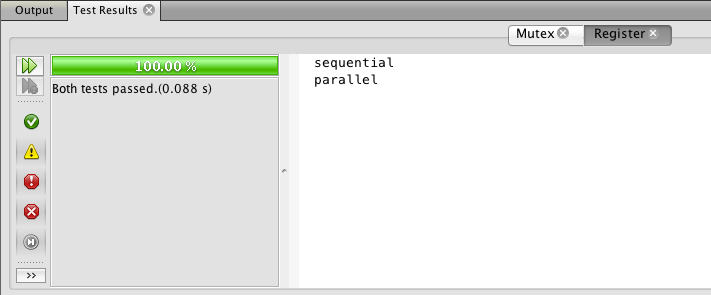
\includegraphics[width=13cm]{WFS00.png}
  \caption{Successful execution of the tests for Wait-Free Snapshot}
  \label{fig:WFS00}
\end{figure}
\par
\begin{figure}[h]
  \centering
  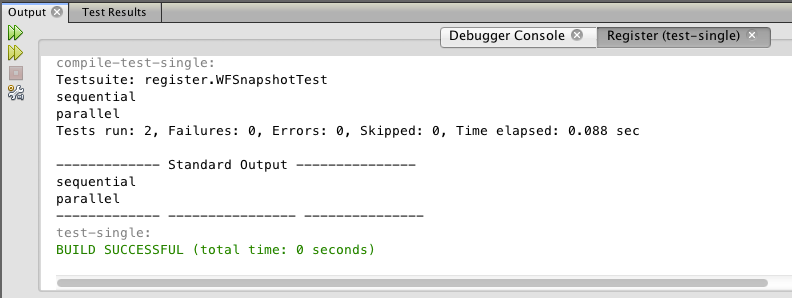
\includegraphics[width=13cm]{WFS01.png}
  \caption{Successful execution of the tests for Wait-Free Snapshot}
  \label{fig:WFS01}
\end{figure}
\par
% ---------------------------------------------------------------------------- %
\subsection{Interpretation}
% ---------------------------------------------------------------------------- %
In this experiment we were able to observe how a Wait-Free Snapshot can be
constructed. 
